Applications which monitor geodynamics using wireless sensor networks have been attempted before. However, most have been used to
monitor volcanic activity, tsunamis and building structure integrity but there are seldom any references of attempts to monitor 


\begin{figure}[ht] \centering
  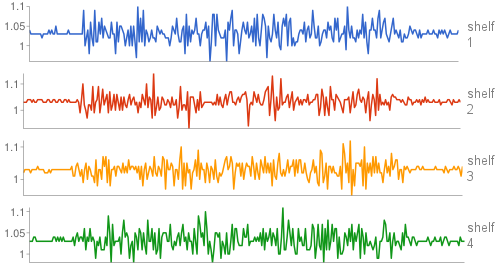
\includegraphics[width=0.5\textwidth]{img/2v.png}
  \caption{Results for the shake table at 2V}
\end{figure}

\begin{figure}[ht] \centering
  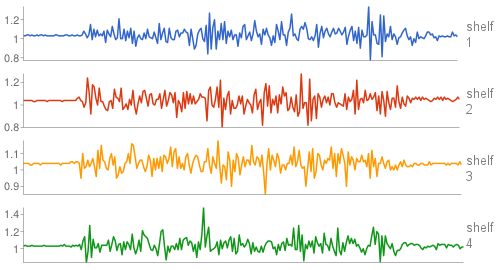
\includegraphics[width=0.5\textwidth]{img/4v.png}
  \caption{Results for the shake table at 4V}
\end{figure}

\begin{figure}[ht] \centering
  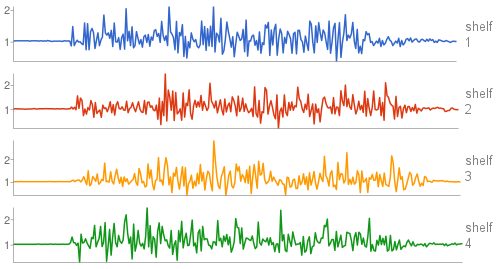
\includegraphics[width=0.5\textwidth]{img/7v.png}
  \caption{Results for the shake table at 7V}
\end{figure}

